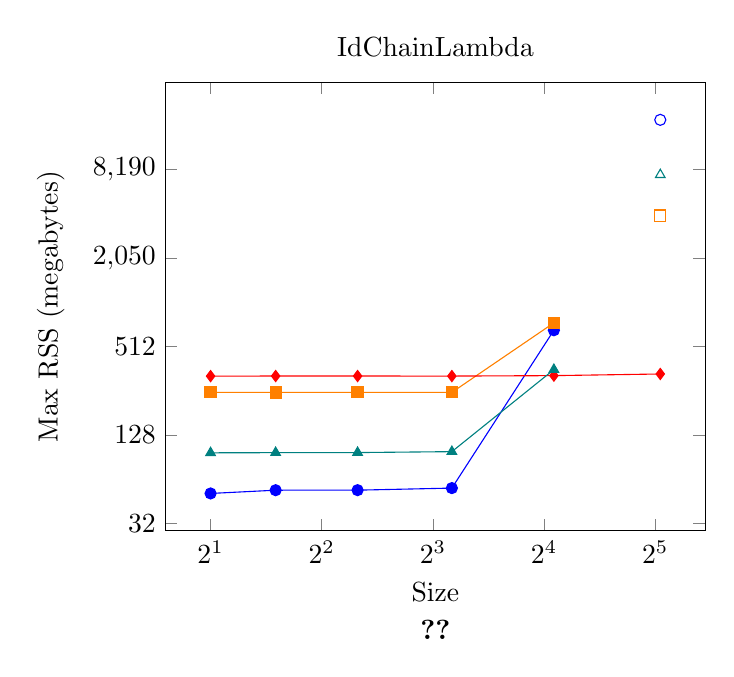
\begin{tikzpicture}
\begin{axis}
[title=IdChainLambda,
xlabel={Size},
ylabel={Max RSS (megabytes)},
legend to name=legend,
legend columns=2,
xmode=log,
log basis x={2},
ymode=log,
log basis y={2},
yticklabel={
  \pgfkeys{/pgf/fpu=true}
  \pgfmathparse{pow(2,\tick)}
  \pgfmathprintnumber[fixed relative,precision=3]{\pgfmathresult}
  \pgfkeys{/pgf/fpu=false}
}]
\addplot [
color=blue,
mark=o,
only marks,
forget plot
] coordinates {
(33.0,17885.913088) 
};
\addplot [
color=orange,
mark=square,
only marks,
forget plot
] coordinates {
(33.0,3986.857984) 
};
\addplot [
color=red,
mark=diamond,
only marks,
forget plot
] coordinates {

};
\addplot [
color=teal,
mark=triangle,
only marks,
forget plot
] coordinates {
(33.0,7560.933376) 
};
\addplot [
color=blue,
mark=*
] coordinates {
(17.0,659.70176) 
(9.0,55.472128) 
(5.0,53.706752) 
(3.0,53.669888) 
(2.0,51.003392) 
};
\addlegendentry{Agda}
\addplot [
color=orange,
mark=square*
] coordinates {
(17.0,740.88448) 
(9.0,248.926208) 
(5.0,248.803328) 
(3.0,248.717312) 
(2.0,248.823808) 
};
\addlegendentry{Idris 2}
\addplot [
color=red,
mark=diamond*
] coordinates {
(33.0,332.201984) 
(17.0,323.739648) 
(9.0,321.470464) 
(5.0,321.712128) 
(3.0,321.683456) 
(2.0,321.31072) 
};
\addlegendentry{Lean 4}
\addplot [
color=teal,
mark=triangle*
] coordinates {
(17.0,355.852288) 
(9.0,98.267136) 
(5.0,96.84992) 
(3.0,96.714752) 
(2.0,96.456704) 
};
\addlegendentry{Rocq}
\end{axis}
\node[anchor=north] at (current axis.below south) {\ref{legend}};
\end{tikzpicture}
